\chapter{Learning from Monolingual Data}
\label{chap:monolingual}
While in this work our target languages are under-resourced, we have many
resources available for the source languages. We would like to use these to
make better sense of the input text, giving our classifiers clearer signals and
better representations for lexical selection in the target language. The
approaches considered in this chapter make additional features or different
representations available to the CL-WSD classifiers based on knowledge of the
source language, either gleaned through unsupervised methods or baked into
extant tools. Since we have relatively little bitext available for
Spanish-Guarani and Spanish-Quechua, we will need to lean more on our Spanish
resources, software and data, in order to make better sense of the input text.

Perhaps most saliently for Spanish, we have abundant monolingual text
available, which suggests that we could use unsupervised methods to discover
regularities in the language, yielding better features for our classifiers.
This approach has been broadly successful in the literature
\cite{turian-ratinov-bengio:2010:ACL,baroni2014don}, and here we adapt some of
the methods explored in previous work on text classification to our task.

Concretely, in this chapter we explore labels learned from existing NLP tools
such as off-the-shelf taggers and parsers for Spanish, Brown clustering
\cite{brown1992class}, and two related approaches to neural embeddings. There
are of course other related methods that one could investigate, especially
making use of the broader literature on distributional semantics, but these
will be left to future work. First we will describe the methods used in some
detail, and then towards the end of the chapter, in Section
\ref{sec:monolingual-experiments}, we describe experiments and present
experimental results.

\section{Monolingual features from other NLP tools}
There are a large number off-the-shelf NLP tools available for Spanish; here we
will look into POS taggers and syntactic parsers specifically. Tagging can help
us capture abstractions over particular word types, and provides some
disambiguation on its own\footnote{For example, perhaps a noun in the window
surrounding a focus word is indicative of a particular meaning. More
concretely, we could imagine the CL-WSD system benefitting from distinguishing
the Spanish \emph{poder} as the infinitive verb ``to be able" from the noun
interpretation ``power, ability".}. Similarly, syntactic structure may also
provide useful features; a verb may have a drastically different translation
in the target language based on its objects.

In the Chipa software, we can make use of arbitrary annotations for the input
text (see Section \ref{sec:annotations}), so adding more features based on
analysis by external tools is straightforward.

As a first step, we synthesize features based on the part-of-speech tags of the
tokens in a window around the current focus word, and using a syntactic parser,
the heads and children of the current focus word. In principle, we could use
other annotations, such as sense annotations from a monolingual WSD system,
given a good one. This idea is akin to one that we will explore in Chapter
\ref{chap:multilingual}, in which we use Chipa itself (trained for other
language pairs, and with larger data sets) to provide annotations, effectively
using some other target language as a tagset for WSD.

For POS tagging, we run the open source FreeLing text analysis suite
\cite{padro12} on input sentences. FreeLing can perform a number of analyses
for Spanish, including POS tagging, dependency parsing, lemmatization, and
named entity recognition, of which the latter two are part of the standard
preprocessing done for all experiments in this work. When all the text for an
experiment is known beforehand, as in the experiments reported in this chapter,
we can run FreeLing during the data annotation step (see Section
\ref{sec:datasetsandpreprocessing}) and simply record FreeLing's output as
additional features. When running on novel test sentences, as in server mode,
we must run it on those sentences just before inference time.

Similarly, for syntactic features, we use MaltParser\cite{Nivre06maltparser:a}
\footnote{Available at \url{http://maltparser.org/} ; in this work we use
version 1.9.0 of the parser, and the ``espmalt" pretrained model, which is
available at \url{http://www.iula.upf.edu/recurs01_mpars_uk.htm}, and was
trained on the IULA Treebank\cite{MARIMON12.519}, by researchers from the IULA
group at Universitat Pompeu Fabra.} to get dependency parses of the input
sentence. This is also performed as a corpus annotation, making the syntactic
relationships for each token available during feature extraction. The parser
here depends on the POS tags produced by FreeLing. Thankfully, they use the
same tag set, but as with any pipeline of NLP systems, using the inferred
output from the tagger as input to the parser carries the risk that errors at
early stages in the pipeline could propagate and cause problems at the later
stages of processing\footnote{Here we note this concern but move on; it is a
very general problem, and solutions to it are an open area of research.}.  The
parser also depends on the coarse-grained ``universal" POS tags
\cite{PETROV12.274}, which we manually map from the IULA tagset to universal
coarse tags.

Operationally, before training our CL-WSD system we parse all of the training
data with the given MaltParser model and the tags inferred by FreeLing during
preprocessing. The parses output by MaltParser are stored on disk in CONLL-X
format. Then with a corpus annotation script, we use the saved parses to find
every token's syntactic head (or the root of the sentence), and every token's
syntactic children, if any. All of these are marked in the annotated training
data, to be made available during feature extraction. During feature extraction,
chipa turns these stored annotations into sparse binary features. The list of
all syntactic features made available to the classifier is listed in Figure
\ref{fig:syntacticfeatures}.

%% XXX: maybe make a diagram for an example of how that works?
\begin{figure*}
  \begin{centering}
  \begin{tabular}{|r|p{11cm}|}
    \hline
    name          & description  \\
    \hline
    \texttt{postag}    & part-of-speech tag for the focus token \\
    \hline
    \texttt{postag\_left}  & POS tag for the token to the left of focus token \\
    \hline
    \texttt{postag\_right} & \emph{ibid.}, for the right \\
    \hline
    \texttt{head\_lemma} & lemma of the focus word's syntactic head, or ROOT if
    it has no head). \\
    \hline
    \texttt{head\_surface} & \emph{ibid.}, but for the syntactic head's surface
    form. \\
    \hline
    \texttt{child\_lemma} & lemma of the syntactic child or children of the
    focus word. Feature appears multiple times for multiple children. \\
    \hline
    \texttt{child\_surface} & \emph{ibid.}, but for the children's surface
    forms. \\
    \hline
  \end{tabular}
  \end{centering}
  \caption{Additional syntactic features}
  \label{fig:syntacticfeatures}
\end{figure*}

\section{Brown Clustering}
The Brown clustering algorithm\cite{brown1992class}, also known as IBM
clustering, as it was developed by the Candide group at IBM, takes an
unannotated text corpus as input and assigns each word type found the corpus
into hierarchical clusters such that types in the same cluster have similar
usage patterns, according to the bigram statistics of the corpus. The tree of
clusters is binary-branching, so the name of a cluster is simply its path from
the root of the tree.  The desired number of ``leaf" clusters must be set ahead
of time, as a tunable parameter.

We can use this clustering to create more features for our classifiers,
considering the clusters into which a word type falls as a tag for instances of
that word. These annotations describe a more abstract, less sparse
representation than surface forms or lemmas, hopefully providing useful
semantic and syntactic generalizations.

Brown clustering uses greedy optimization to find cluster assignments. Each of
the word types present in the input corpus must be placed into one of a fixed
number of hierarchical clusters, such that the assignment attempts to maximize
the probability of the input corpus.  As the original intention of the approach
was for class-based language models, the scoring function is the mutual
information between two immediately subsequent tokens (i.e., a bigram).
Concretely, the optimization process is searching for a clustering $C$ that
maximizes the probability of the corpus $\boldsymbol{w}$, according to the
formula in Figure \ref{fig:brownprob}.

\begin{figure*}

  \begin{equation} \label{eq:brownclassprob}
  P(\boldsymbol{w}; C) = \prod_{w_i} p(w_i | C(w_i)) p(C(w_i) | C(w_{i-1}))
  \end{equation}

  \caption{The Brown clustering expression for the probability of a corpus with
  a specific clustering $C$. It is the product, for each token, of the
  probability of that token given its cluster, and the probability of that
  current cluster given the previous cluster. This is analogous to the
  ``emission" and ``transition" probabilities used in an HMM-based tagger.}
  \label{fig:brownprob}
\end{figure*}

Finding the globally optimal assignment turns out to be an intractable problem,
but several greedy approaches that find local optima have been explored in the
literature.  Notably, in addition to Liang's approach, Franz Och's
\texttt{mkcls} package (familiar to Moses users, and described in
\cite{och1999efficient}) optimizes the same function. In any case, with the
available software running on modern hardware, we can find a clustering for the
corpora used in this work in a fairly short time -- a few hours at most.

In applying Brown clustering to this task, we would like to answer several
questions.

\begin{itemize}
  \item Can learning Brown clusters from  monolingual source-text resources 
    improve our performance on this CL-WSD task?
  \item Does more source-language text help us learn more helpful Brown
  clusters, with respect to the CL-WSD task?
  \item How does the genre of the input text affect our performance, and how
  does this relate with the size of the text? Is there a size at which we
  can learn a better clustering that overcomes genre mismatches?
  \item What kinds of preprocessing should we do on the source text? Most
  saliently, should the source text be lemmatized? We might expect that Brown
  clustering will help us find abstractions over syntax, but perhaps
  lemmatization would help it find more semantic abstractions in practice. Or
  perhaps it would be more effective to use the same input corpus in both
  lemmatized and inflected forms.
\end{itemize}

We can use such a clustering $C$ (i.e., a mapping from word types to clusters)
to extract a number of different kinds of features for our classifiers; we may
also choose a variety of inputs to the clustering algorithm in the first place.
In principle, we may gain useful clusters from any large sample of text in the
source language, and any preprocessing on that corpus could be useful.
%% XXX: working here

We tried, for example, dropping a bag of all the clusters that occur in the
sentence, and prefix features for all the clusters that appear too!

It might be the case that we really just need to add the very local context --
three words on a side? In Turian et al, they do two words on a side.

%% XXX: we have versions for wikipedia and europarl, don't we?
\begin{figure*}
  \begin{centering}
  \begin{tabular}{|r|p{11cm}|}
    \hline
    name          & description  \\
    \hline
    \texttt{brown\_bag}    & Bag of all Brown clusters for the entire sentence \\
    \hline
    \texttt{brown\_window}  & All Brown clusters for a window around the focus word\\
    \hline
    \texttt{flat\_brown\_bag} & \emph{ibid.}, ... \\
    \hline
    \texttt{flat\_brown\_window} & \emph{ibid.}, ... \\
    %% XXX: add some more
    \hline
  \end{tabular}
  \end{centering}
  \caption{Features extracted from Brown clusters}
  \label{fig:brownfeatures}
\end{figure*}


\section{Brown clustering in practice}
In this work we use Percy Liang's implementation \footnote{Available at
\url{https://github.com/percyliang/brown-cluster}} of Brown clustering
\cite{Liang05semi-supervisedlearning}.
We have run the tool on several corpora, varying in size from the Bible
(roughly 30K sentences), to the larger Europarl corpus \cite{europarl} (2
million sentences), to larger still, a dump of the Spanish-language Wikipedia
(20 million sentences). When working with Spanish, a consideration is the
relative morphological richness of our input text; we could choose to lemmatize
our input text before clustering, or not, and this decision will be more
significant than it would be for English, given how much more inflection is
present in Spanish.

In this work we try both approaches, running the clustering tool on both the
lemmatized and inflected versions of our input corpora. Examining the learned
clusters, we see a few interesting things; first note the semantic
relatedness. Also note that in the clusters learned from the surface-level
text, we pick up on syntactic regularities as well as semantic ones.

%% when we do clustering on lemmas, we seem to pick up more on ``semantic"
%% categories of things. Note the ``infrastructure" cluster below -- it's got
%% words that all pertain to infrastructure!

%% TODO: include examples of the clusters that we learn from different corpora
%% specify lemmatized versus not lemmatized


When we don't use lemmas, the cluster that contains ``infraestructura" contains
these words: \emph{formación educación tecnología infraestructura publicidad
enseñanza ocupación religión vivienda ética propaganda banda fusión huelga
creatividad medicina manipulación tribuna cualificación comida}. It seems like
this is more about grammatical gender: those are all singular feminine nouns.

In fact, the words in many of the clusters all seem to have the same
grammatical gender and number. To get more semantic similarity, maybe we should
cluster on lemmas -- otherwise the morphological features of Spanish could
overwhelm the clustering approach.

\TODO{replace with current example}
\begin{figure*}[t!]
  \begin{tabular}{|r|p{10cm}|}
    \hline
    category  & top twenty word types by frequency \\
    \hline
    countries & francia irlanda alemania grecia italia españa rumanía portugal polonia suecia bulgaria austria finlandia hungría bélgica japón gran\_bretaña dinamarca luxemburgo bosnia \\
    \hline
    more places & kosovo internet bruselas áfrica iraq lisboa chipre afganistán estrasburgo oriente\_próximo copenhague asia chechenia gaza oriente\_medio birmania londres irlanda\_del\_norte berlín barcelona \\
    \hline
    mostly people & hombre periodista jefes\_de\_estado individuo profesor soldado abogado delincuente demócrata dictador iglesia alumno adolescente perro chico economista gato jurista caballero bebé \\
    \hline
    infrastructure & infraestructura vehículo buque servicio\_público cultivo edificio barco negocio motor avión monopolio planta ruta coche libro aparato tren billete actividad\_económica camión \\
    \hline
    common verbs & pagar comprar vender explotar practicar soportar exportar comer consumir suministrar sacrificar fabricar gobernar comercializar cultivar fumar capturar almacenar curar beber \\
    \hline
  \end{tabular}
\caption{Some illustrative clusters found by the Brown clustering algorithm on
the Spanish Europarl data. These are five out of $C=1000$ clusters, and
were picked and labeled by hand. The words listed are the
top twenty terms from that cluster, by frequency.}
\label{fig:clusters}
\end{figure*}

Figure \ref{fig:clusters} shows some illustrative examples of clusters that
we found in the Spanish Europarl corpus.  Examining the output of the
clustering algorithm, we see some intuitively satisfying results; there are
clusters corresponding to the names of many countries, some nouns referring to
people, and common transitive verbs. Note that the clustering is unsupervised,
and the labels given are not produced by the algorithm.

We additionally show the effects on classification accuracy of adding features
derived from Brown clusters, with clusters extracted from both the Europarl
corpus and the Spanish side of our training data.
We tried several different
settings for the number of clusters, ranging from $C=100$ to $C=2000$.
In all of our experimental settings, the addition of Brown cluster features
substantially improved classification accuracy. We note a consistent upward
trend in performance as we increase the number of clusters, allowing the
clustering algorithm to learn finer-grained distinctions.
The training algorithm takes time quadratic in the number of clusters,
which becomes prohibitive fairly quickly, so even finer-grained distinctions
may be helpful, but will be left to future work. On a modern Linux
workstation, clustering Europarl (~2M sentences) into 2000 clusters took
roughly a day.

The classifiers using clusters extracted from the Spanish side of our bitext
consistently outperformed those learned from the Europarl corpus. We had an
intuition that the much larger corpus (nearly two million sentences) would
help, but the clusters learned in-domain, largely from the Bible, reflect
usage distinctions in that domain. Here we are cheating slightly, as
information from the complete corpus is used to classify parts of that corpus;
the results here should be considered an upper bound on what would be possible
with matching domain, if we are willing to trade size for a good match, rather
than as clean experimental results.

\section{Neural Word Embeddings}
Another rich source of features that has proved useful for many text
classification problems in recent years is neural word embeddings, perhaps most
famously developed in the work of Mikolov et al. \cite{mikolovword2vec} and
their associated open source implementation of the technique,
word2vec\footnote{Available at
\url{https://code.google.com/archive/p/word2vec/}}. In this work we investigate
the use of ``word2vec"-style word embeddings, as well as the related technique,
``doc2vec" or ``paragraph vectors"
\cite{dai-document-embedding-2015,quocle-distributed-representations-2014}.
These techniques let our classifiers operate on lower-dimensional dense vectors
(of a few hundred dimensions, typically), as opposed to the high-dimensional
and sparse vectors typically used in earlier NLP literature\footnote{
What we might consider to be ``symbolic" binary features used in machine
learning systems for NLP in recent decades -- such as ``the word `dog` appears
in the sentence" -- are effectively equivalent to these very sparse ``one hot"
representations of words, in which, for a vocabulary of size $|V|$, words are
represented by a length-$V$ vector in which all but one of the elements are 0}.

There is a rich literature on continuous representations for words; the idea
has a long lineage in NLP, and we could try any number of dimensionality
reduction or distributional semantics approaches here. Recent empirical work by
Baroni et al \cite{baroni2014don} (summed up by the title of the paper, ``Don't
Count, Predict!") has shown that representations built during discriminative
learning tasks are typically more effective for text classification problems
similar to ours.

Unlike Brown Clustering, which infers hierarchical clusters for each word type,
but like other embedding techniques, word2vec learns multidimensional
representations for word types, turning the very sparse ``one hot"
representation in which a words with similar uses or meanings do not have any
obvious similarity into a much denser continuous space in which words with
related meanings are placed nearby. These ``embeddings", or placements of word
types into a continuous space, are learned during some other classification
task, and are performed by the early layers of a neural network.

The word2vec model in particular has two variations, useful in different
contexts. One, called Continuous Bag-of-Words (CBOW) learns a classifier that
can predict individual words based on their context, while the ``skip-grams"
variant does the reverse and learns to predict context words based on an
individual focus word. The received wisdom\footnote{According to the TensorFlow
tutorial on word2vec, available at
\url{https://www.tensorflow.org/tutorials/word2vec}} is that CBOW is more
appropriate when training on smaller data sets, but this is an empirical
question and here we try out both variants.

In either case, running a word2vec training process results in a static mapping
from word types to their embeddings in a vector space of a given size,
typically a few hundred dimensions. These embeddings have been shown to be
helpful as features in a number of different NLP tasks \cite{baroni2014don},
allowing us to learn richer representations of word types from plentiful
unannotated monolingual text. This effectively turns what was a purely
supervised task, requiring labeled training data, into a semi-supervised task,
in which the representation-learning phase can be carried out on unlabeled data
by synthesizing a supervised learning task that can be performed with simple
monolingual text as its training data.

We trained a variety of word2vec embeddings for our text classification tasks,
training on the Spanish-language section of the Europarl corpus (roughly 57
million words and 2 million sentences) and a dump of Spanish Wikipedia (449
million words, 20 million sentences). We learned embeddings using both CBOW and
skip-gram approaches, in 50, 100, 200, and 400 dimensions. In all cases, we
used the associated \texttt{word2phrase} tool, distributed with the initial
\texttt{word2vec} implementation, which finds collocations in the input text
and treats them as individual tokens. The same collocations must be identified
in the input text for their embeddings to be used. At lookup time, we keep a
list of all the multiword expressions present in the dictionary of embeddings,
sorted from longest to shortest, first considering number of tokens, then
breaking ties by considering number of characters, and greedily replace any of
these multiword expressions (starting with the longest) found in the input text
with the token representing that MWE.

\subsection{From word embeddings to classification features}
We should note that the embeddings learned for a word type are fixed for that
word type, and do not reflect the context of a particular token, so a focus
word's embedding vector will not provide useful classification features on its
own. This leaves us with the problem of how to make use of the word vectors in
a given sentence. Concretely, we must decide how to combine several word
vectors together, and which word vectors in a sentence to choose for
combination. The typical approach (XXX citation) is to take element-wise sums
or averages over the embedding vectors for the tokens in a context.

There are a variety of approaches we could take, even within summing and
averaging. We could sum (element-wise) all of the word vectors for all the
tokens in the entire sentence. We could only consider the words in a narrow
window around the focus word. Or we could perform a weighted sum, in which
words nearer to the focus word are given more weight, but these weights drop
off according to some function, scaling with the distance from the focus word.
For our experiments here, we try these three different approaches, resulting in
three different feature sets.

In the first feature set, called ``window", we present the classifier with the
element-wise sum of the vectors for the focus word (or the token containing the
focus word, if it is inside a multi-word expression) and the three tokens on
either side. The resulting vector thus has the same dimensionality as the word
embeddings that we learned. Secondly, in the ``fullsent" feature set, we
perform an unweighted element-wise sum of the word embeddings for the entire
sentence. Finally, in the ``pyramid" feature set, we sum the embeddings for
each token in a broad window around the focus word, but before summing, scale
the embeddings by $1.0 - (0.1 * d) $, for a minimum of 0.

%% XXX working here

%% XXX add some citations for papers where people use word embeddings as
%% features

\section{Neural Document Embeddings}
The same researchers that produced word2vec and their collaborators have also
developed approaches that build representations for sequences of text, rather
than individual word types, described in
\cite{dai-document-embedding-2015,quocle-distributed-representations-2014}.
This approach, called ``paragraph vectors" or ``doc2vec" takes unlabeled text
and learns representations for word types jointly with representations for each
\emph{document}. Here a ``document" is an arbitrary sequence of tokens, perhaps
a single sentence, or perhaps much longer, depending on the intended
application.

Similar to word2vec, here doc2vec uses a neural network with a single hidden
layer to predict words in the current context. Here however, the hidden layer
contains not only an embedding trained for word types, but also an embedding
for the current document. Training proceeds by loading the current
representation for the current word and the current document, attempting to
predict some other word in the context (analogous to training for word2vec),
and then updating both representations based on the gradients between the
desired output and the actual output. 

Also similar to word2vec, there are two variants of the approach that can be
used for training. One variant of doc2vec, the ``Distributed Memory Model of
Paragraph Vectors", uses a paragraph embedding combined with word embeddings
for several words in the current context to predict a single individual word.
The other variant, the ``Distributed Bag of Words model of Paragraph Vectors",
simply uses the current paragraph vector to predict all of the words in the
current context, which despite containing ``bag of words" in its name, is more
closely analogous to the skip-gram artitecture for word2vec
\cite{quocle-distributed-representations-2014}, since the model is trained to
predict the entire context based on a single embedding.

In either case, the resulting stored model is the set of embeddings for
individual word types. The embeddings for any particular document in the
training set are not stored, since that document is unlikely to appear again at
inference time, but the embeddings for individual word types provide a useful
generalization, since they constrain embeddings for new documents.

At inference time, doc2vec produces new vectors describing previously unseen
documents based on these fixed word embedding vectors. In our work, as in many
text classification tasks, documents will be input sentences, or perhaps
sentence-length Bible verses. To produce a representation for a new document,
the embeddings for word types are held constant and we run the optimization
process (stochastic gradient descent) to infer an embedding for the current
document, such that it helps predict words in the current context.

doc2vec thus provides a straightforward approach for learning to produce
representations of new documents, based on an unlabeled training corpus. Here
we use the implementation of doc2vec provided by the gensim package
\cite{rehurek-lrec}, with its default settings, which means that training is
carried out with the ``distributed memory" model.
During training data annotation, we take each source-language sentence and
infer a new embedding for it based on a doc2vec model trained on 20 million
sentences dumped from the Spanish-language wikipedia. These sentence-level
embeddings are stored as a token annotation on the first token of each
sentence, so they can be made available during feature extraction.

\section{Experiments}
\label{sec:monolingual-experiments}
Here we repeat the experiments from Chapter \ref{chap:baseline} for
Spanish-Guaraní and Spanish-Quechua, with the addition of features extracted
from syntactic tools, Brown clusters, and the various kinds of neural
embeddings presented in this chapter.

Most of the experiments here used the features in Figure
\ref{fig:baselinefeatures}, but we additionally did experiments with the neural
embedding features on their own.

While there are many possible combinations of these features, we did not try
all of them exhaustively.

\begin{itemize}
  \item es-gn, es-qu with pos tags
  \item es-gn, es-qu with pos tags and syntactic heads and children
\end{itemize}

\begin{itemize}
  \item es-gn, es-qu with europarl brown clusters
  \item es-gn, es-qu with wikipedia brown clusters
  \item es-gn, es-qu with word2vec embeddings of dimensions (50, 100, 200, 400)
  from both europarl and wikipedia
\end{itemize}

\begin{itemize}
  \item es-gn, es-qu with europarl embeddings
  \item es-gn, es-qu with wikipedia embeddings
\end{itemize}

\begin{itemize}
  \item combine the most promising ones
  %% XXX: we don't actually have code to combine word2vec features with the
  %% sparse features yet.
\end{itemize}

\section{Classification Results} 

\begin{figure}
  %% 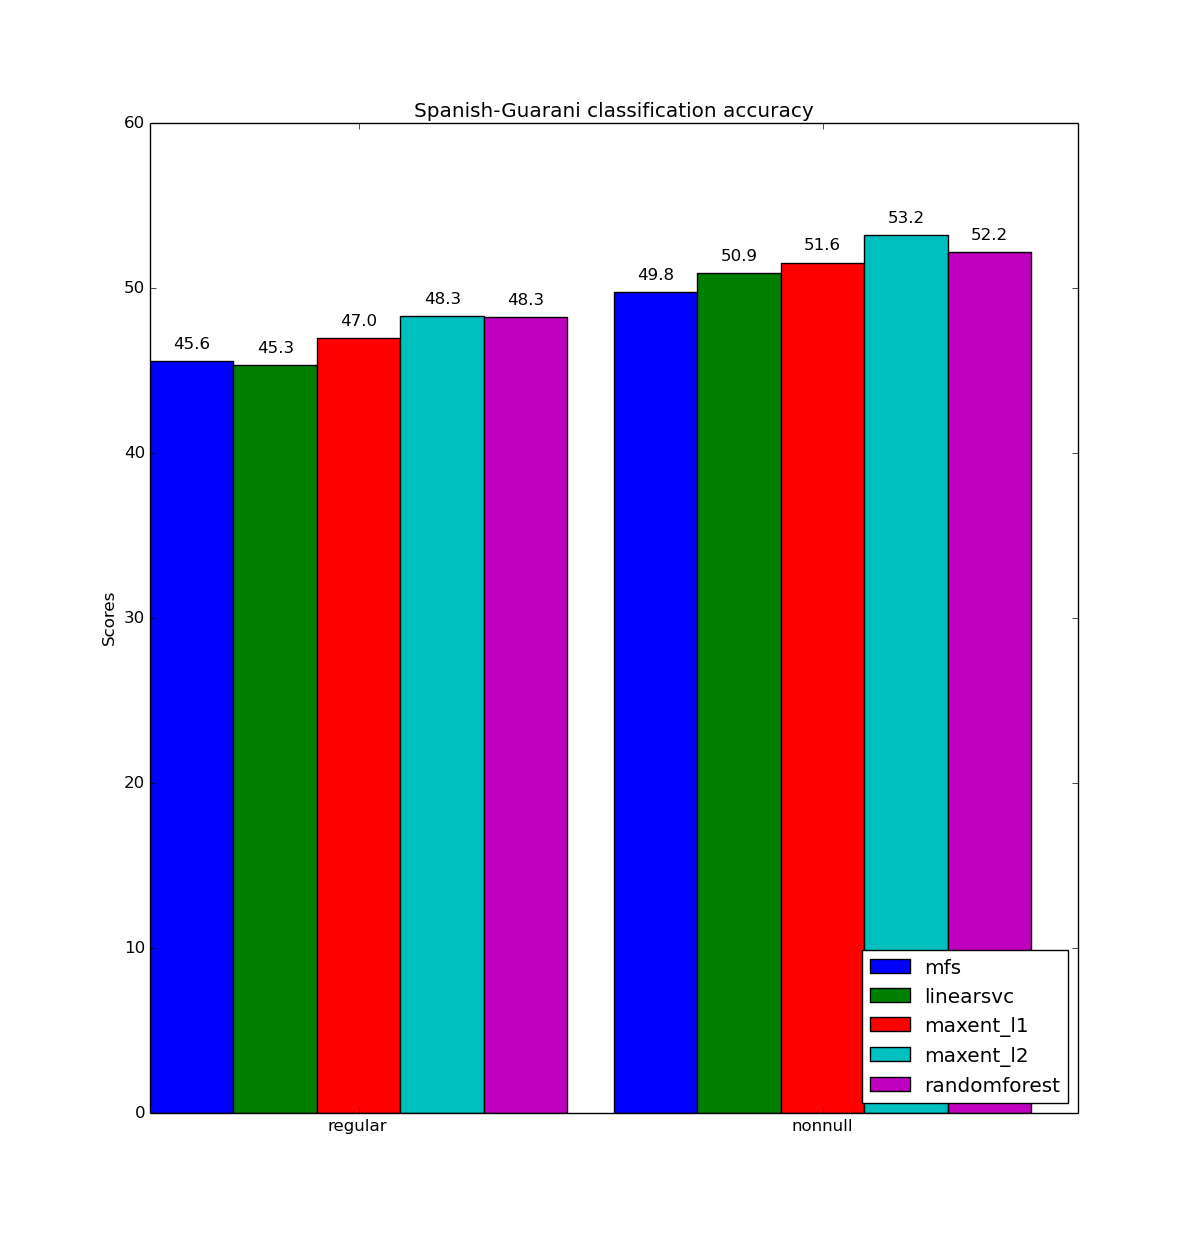
\includegraphics[width=\textwidth]{baseline-esgn-ch4.png}
  \caption{Baseline Chipa scores for Spanish-Guarani, by classifier.}
  \label{fig:esgnresults:monolingual}
\end{figure}

\begin{figure}
  %% 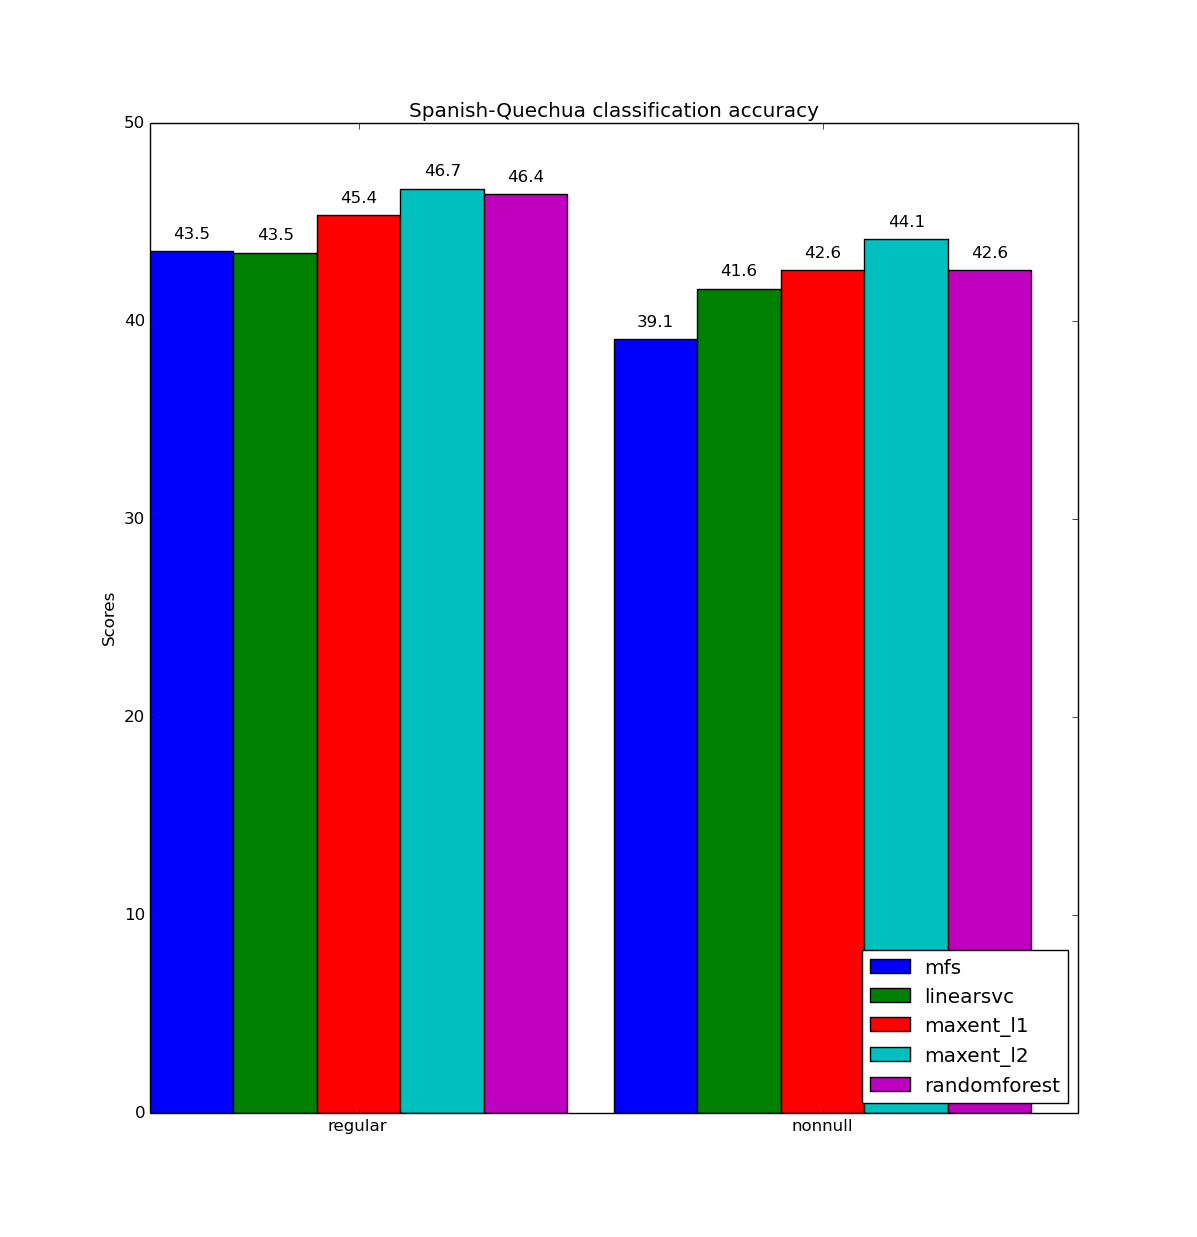
\includegraphics[width=\textwidth]{baseline-esqu-ch4.png}
  \caption{Baseline Chipa scores for Spanish-Quechua, by classifier.}
  \label{fig:esquresults:monolingual}
\end{figure}

\subsection{Results: adding syntactic features}
Taking a look at the scores from the features based on easily available
Spanish-language taggers and parsers, we see that for Spanish-Guarani, we were
able to surpass the MFS baseline with the dependency-parse and POS-tag-based
features. They seemed to work especially well with the L2-norm maxent
classifier and random forests.  Furthermore, they beat the default features
described in Chapter \ref{chap:baseline} by roughly half a percentage point:
0.5 or 0.6 percentage points, in the ``regular" and ``non-null" settings,
respectively. Adding the part-of-speech features without the parse features
worked nearly as well, falling a tenth of a percentage point behind using all
of the syntactic features in the ``regular" setting, and three tenths of a
point behind in the ``nonnull" setting.

We see fairly similar results for Spanish-Quechua, which are shown in Figure
\ref{fig:esquresults:monolingual}. Our strongest results for the ``regular"
classification setting came with the use of the syntactic features, using
random decision forests, which beat the Spanish-Quechua MFS baseline by 3.5
percentage points. Random forests with the ``POS tags" feature set was nearly
as strong, beating the baseline by 3.1 points. Random forests seemed to work
quite well broadly for Spanish-Quechua; the default feature set beat the
MFS baseline by 2.8 points.

Maximum entropy classifiers with L2 regularization and syntactic features also
did fairly well for Spanish-Quechua, beating the baseline by 2.9 points.

For the ``nonnull" case of Spanish-Quechua, we see the order of the top
classifiers flipped; the maximum entropy classifier had the top results,
beating the MFS baseline by 5 percentage points. Using just the default
features with added POS tags beats the baseline by 4.7 percentage points. For
comparison, the default feautres win out over the MFS baseline by 4 percentage
points with L2 maximum entropy, or 3.9 points with random forests. For random
forests with the syntactic features, we see that setting beat the MFS baseline
by 4.3 points.

%% furthermore: how does our accuracy correlate with training set size, when we
%% consider words separately? Can we draw that curve?

\subsection{Results: adding clustering features}
%% XXX working here
Results for clustering for Spanish-Guaraní:
using a bag of brown for the whole sentence didn't work very well.
Using the brown clusters for a small window around the focus word worked well!

Similar for Spanish-Quechua.

Lemmatizing the source text before extracting
Brown clusters did not seem to help; in fact the scores for lemmatized Brown
clusters were a few tenths of a percentage point lower.  

When we use Brown clusters in the window alongside the syntactic featues, that
works best of all so far, for Spanish-Guaraní and Spanish-Quechua, in both
regular and nonnull settings. That is pretty cool. So if you've got a tagger,
a parser, and a bunch of monolingual text for your source language, you can
probably make your CL-WSD classification rather better, all without any
particular resources for your target language.

\subsection{Results: neural embeddings alone}
In Figure \ref{fig:esgnresults:monolingual}, we see the results for the Chipa
system with roughly the same classifiers used in Chapter \ref{chap:baseline},
but now with the features based on our monolingual resources described in this
chapter, for Spanish-Guaraní. As before, we report classification accuracy
as a percentage, and we performed ten-fold cross-validation, using all of the
available training data for each of the lemmas in a given language pair's
bitext that appear at least fifty times. Also as before, we consider the
``regular" and ``non-null" classification settings separately.

In general, we see that through using the word2vec embeddings summed over a
window surrounding the focus word, we can get results significantly better than
the MFS baseline, although not with all settings and not with all classifiers.
One fairly successful combination seems to be the skipgram embeddings trained
on the Wikipedia dump, with a window size of three tokens on either side of the
focus word, which beats the MFS accuracy by 1.2 percentage points over all
words for the nullable ``regular" setting, and 1.4 percentage points in the
``non-null" setting. The width of the embeddings trained seems to have little
effect, but the top performances were seen in both settings with the skipgrams
trained on Wikipedia. We also see that the clear winner, out of the classifier
architectures tried, was the maximum entropy classifier with L1 regularization.
The same linear classifier with L2 regularization was also able to outperform
the MFS baseline, but not as well as the L1 version.

Additionally, using the ``pyramid" style of embedding combinations seems to
slightly outperform simply summing over a window of three tokens. Out of all
the results for Spanish-Guaraní using only neural embeddings, we got the best
results using ``pyrmaid" style combinations, with the Wikipedia skipgram
embeddings, and a maximum entropy classifier with L1 regularization. This beat
the MFS baseline by 1.3 percentage points in the ``regular" setting and 1.5
percentage points in the ``nonnull" setting, slightly outperforming the
``window" style of combination.

Using skipgram embeddings trained on the smaller Europarl corpus was also able
to beat the MFS baseline, but by a smaller margin than the embeddings trained
on Wikipedia.

Approaches that did not beat the MFS baseline included all uses of continuous
bag of words, classifiers other than maximum entropy, and summing the
embeddings across the entire sentence. Additionally, while they were able to
roughly match the MFS baseline, the doc2vec word embeddings were not able to
outperform that baseline. Intuitively, perhaps trying to capture the entire
sentence, rather than the area around the focus word, is less helpful for
making local CL-WSD decisions; this interpretation is consistent at least with
our observation that summing the embeddings for the entire sentence is less
helpful than summing the embeddings in a small window around the focus word.

For Spanish-Quechua, we were also able to beat the MFS baseline using only word
embedding features. Here again, we see the use of ``pyramid" combinations
working well, and the Wikipedia embeddings outperforming the embeddings trained
on Europarl. The top combination for Quechua on the ``regular setting", using
100-dimensional skipgram embeddings trained on Wikipedia, combined with the
``pyramid" approach, beats the MFS baseline by 1.8 percentage points. The other
dimensionalities follow closely behind, with 200, 100, and 400 providing
results just a few tenths of a percent worse. Also, the ``window" combination
method worked nearly as well as ``pyramid".

In the ``nonnull" setting, using word embedding features alone also beats the
MFS baseline, this time by 3.5 percentage points, using pyramid combinations,
and 400-dimensional skipgram embeddings trained on Wikipedia, with the L2
maximum entropy classifier. The other dimensionalities follow closely behind,
as do the ``window" combination methods.

As with the previous language pair, for Spanish-Quechua using skipgram
embeddings was much more effective on this task than the continuous bag of
words embeddings; we were unable to surpass the MFS baseline with any of the
``cbow" embeddings, whether they were trained on Europarl or Wikipedia, and for
any of the combination methods. Also, as with Spanish-Guaraní, we did not see
the ``fullsent" combination strategy beat the MFS baseline for any of our
parameter settings.

%% XXX: make some nice graphs

\section{Results: combining neural embeddings with sparse features}

%% XXX: still need to implement this and run the experiments!!
